% EPL master thesis cover template
\documentclass{eplmastersthesis}

% Imports
\usepackage{multicol}
\usepackage{multirow}
\usepackage{rotating}
\usepackage{hyperref}
\usepackage{float}
\usepackage{forest}
\usepackage{amsmath}
\usepackage{setspace}
\usepackage{titlesec}
\setcounter{secnumdepth}{4}

\graphicspath{{F:/Memoire/CodeSavedOnline/New/MasterThesis/paper/FirstVersion/Graphs/}}

% Fill in here the information: title, student name, speciality, jury members
\title{CP based Sequence Mining on the cloud using spark}	% Master thesis title
%\subtitle{Subtitle (optional)}			% Optional subtitle
\author{Cyril \textsc{de Vogelaere}}	% Student name
%\secondauthor{Firstname \textsc{Lastname}}	% Second student name if applicable
\speciality{Computer Science}		
% Speciality (use one of the following options):
										% Biomedical Engineering
										% Chemical and Materials Engineering
										% Civil Engineering
										% Computer Science
										% Computer Science and Engineering
										% Electrical Engineering
										% Electro-mechanical Engineering
										% Mathematical Engineering
										% Mechanical Engineering
										% Physical Engineering
%\options{Option(s)}		% If required by program commission mention options
\supervisor{Pierre \textsc{Schaus}}	% 1st supervisor name
%\cosupervisor{Firstname \textsc{Lastname}}	% 2nd supervisor name if applicable
\readerone{John \textsc{Aoga}}		% 1st reader name
\readertwo{Guillaume \textsc{Derval}}		% 2nd reader name
%\readerthree{Firstname \textsc{Lastname}}	% 3rd reader name
\years{2016-2017}	% Academic year
\pagenumbering{arabic}

\newcommand\danger{%
 \makebox[1.4em][c]{%
 \makebox[0pt][c]{\raisebox{.1em}{\small!}}%
 \makebox[0pt][c]{\color{red}\Large$\bigtriangleup$}}}%

\titleformat{\paragraph}
{\normalfont\normalsize\bfseries}{\theparagraph}{1em}{}
\titlespacing*{\paragraph}
{0pt}{3.25ex plus 1ex minus .2ex}{1.5ex plus .2ex}

%\renewcommand{\baselinestretch}{1.15}

\begin{document}

\begin{singlespacing}
\maketitle					% To create front cover page
% To fix footnotes problem
\newgeometry{top=2.5cm,bottom=2.5cm,left=2.5cm,right=2.5cm}
\end{singlespacing}

\tableofcontents
\newpage
\listoffigures
\listoftables
\newpage

\begin{abstract}
TODO - Half a page to a page of content should be enough
\end{abstract}
\newpage


\section{Introduction}

Frequent pattern mining is a widely studied problem concerned with discovering frequent subsequences in a given dataset of sequences, where each sequence is an ordered list of symbols. \\
Those frequent pattern mining (FPM) problems can generally be further differenced into two kinds of problems :

\begin{itemize}
\item Multi-item pattern mining problems, which consist in finding sequences of frequent sets of symbols. While time consuming, this type of FPM is frequently used in the industry. A practical example would be to find sequences of items often bought together, so that long term promotions could be made and sales could be increased.
\item Single-item pattern mining problems, which consist in finding sequences of frequent symbols. While also time consuming, it has been proven through various papers\footnote{Link to references or citation of all such paper ? TODO decide} that algorithms specialised for single-item pattern mining can widely outperform their multi-item counterparts on the same datasets. Motivating their common uses in applications such as web log mining and biological sequence analysis.
\end{itemize}

While many such specialized algorithms exist, constraint programming (CP) has often been proposed as a framework for both single-item and multi-item pattern mining in recent years \cite{CPforDataMining, CPforItemSetMining}. The main benefit of CP based algorithms lying in their modularity, as they allow the addition of various constraints spanning over a wide range of possibilities, such as restriction on symbol occurrences, pattern length, respect of regular expressions, ... \newline

However, it was feared that this increased flexibility came with a performance cost. Many of the developed algorithm staying uncompetitive with state-of-the-art specialized methods. Although many improvements had been made, notably by Kemmar et al \cite{Kemmar_global, Kemmar_gap}, which had further extended this work by introducing one constraint (module) for both the pseudo-projection and the frequency pruning, only reasonable performances were obtained. \newline

However, a recent paper \cite{PPIC}, shattered those fears by out-performing, not only other CP based implementation, but also state-of-the-art specialized methods (see Figure \ref{PPIC's perfomance against other specialized implementations}). This PrefixSpan based algorithm called PPIC, implemented on the open source CP solver OscaR\footnote{\url{https://bitbucket.org/oscarlib/oscar/wiki/Home}}, achieve those performances by combining various ideas from pattern mining, such as the last-position lists of the LAPIN algorithm, as well as ideas from CP, such as trailing which allow faster computations and avoids unnecessary copying. \newline

While extremely performant on single-item pattern mining problems, PPIC still suffer from an important limitation. The developed implementation is not scalable, which is a serious flaw for the industry as cloud computation are often used to solve large problems in a timely fashion. \newline

Through this paper, we shall attack this limitation under various angles and prove that an efficient and scalable CP based FPM algorithms can be developed. Additionally, we will also study possible implementation of a CP based multi-item pattern solver.

\section{Option for Scalability :}

Since the OscaR library currently doesn't allow scalable cloud computation, and that an efficient such implementation couldn't reasonably be made during the short time frame of a master thesis, our first step was to choose a cloud computing library to develop our scalable implementation. \newline

Since, fortunately, FPM problems are embarrassingly parallel problem, we had the opportunity to choose from a selection of widely used open-source libraries. We, however, restricted ourselves to Scala compatible framework, as the CP library supporting PPIC was implemented in this language. Rapidly, we were left to choose from to major options :

\begin{enumerate}
\item Hadoop mapreduce
\item Spark
\end{enumerate}

TODO : Should I make two subsections, one explaining Spark and its concept and one explaining Hadoop ?

Both of those libraries already disposing of a scalable PrefixSpan implementation. It was thus a matter of determining whose performances were better, and whether those implementations could be efficiently extended through CP technologies. \newline

Fortunately for us, performance comparison had already been done in a widely recognised scientific paper on Spark's RDD \cite{RDD}. The performances comparisons they obtained then, are presented in Figure \ref{fig:hadoopVSspark}

\begin{figure}[h]
  \centering
  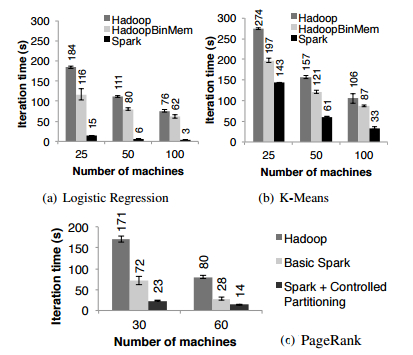
\includegraphics[width=0.6\textwidth]{hadoopVSspark.png}
  \caption{Performance comparison of Hadoop and Spark}
  \label{fig:hadoopVSspark}
\end{figure}

As you can see, performance-wise, Spark vastly outperform Hadoop thanks to its ability to use both in memory and on disk computations. Allowing up to 100x speed-up under the right circumstances, as you can see in the logistic regression problem. According to the official website, Spark would also boast a 10x speed-up through on disk computation, but no performance benchmarks were provided. \newline

In terms of extensions through CP technologies, we quickly realised that Hadoop would be far less practical. Although MapReduce can be used to execute the standard PrefixSpan algorithm, and could certainly be modified to introduce CP elements, Spark can support any coarse-grained transformation with its RDDs. Allowing more precise implementations where only required transformations would be made, instead of simple sequences of Map-Combine-Reduce. \newline

We thus decided to use Spark to implement our scalable version of PPIC.

\section{Solution Correctness - Verification Procedure}

TODO ? (It feels like it would be too much, should I add that ?)

\section{Performance Testing Procedure}

To compare performances, we first need to discuss how they were obtained, and on which dataset they were tested.

\subsection{Performance Testing Datasets}

For our performance tests, eight datasets were chosen for the different characteristic they displayed. The goal being to prove the efficiency of the developed algorithm in a wide range of situations. The chosen datasets and their characteristic are displayed in Table \ref{tab:datasets} : \newline

\begin{table}[h]
  \centerline{
  \begin{tabular}{| c | l | c | c | c | c | c | c | r |}
  	\hline
  	& Dataset & \#SDB & N & avg(\#S) & avg(\#Ns) & max(\#S) & Sparsity & description \\
  	\hline
  	\multirow{6}{*}{1.} 
  	& BIBLE & 36369 & 13905 & 21.64 & 17.85 & 100 & 1.18 & text \\
  	\cline{2-9}  
  	& FIFA & 20450 & 2990 & 36.24 & 34.74 & 100 & 1.19 & web click stream\\
  	\cline{2-9}  
  	& Kosarak-70 & 69999 & 21144 & 7.98 & 7.98 & 796 & 1.0 & web click stream\\
  	\cline{2-9}  
  	& LEVIATHAN & 5834 & 9025 & 33.81 & 26.34 & 100 & 1.25 & text\\
  	\cline{2-9}  
  	& PubMed & 17237 & 19931 & 29.56 & 24.82 & 198 & 1.17 & bio-medical text\\
  	\cline{2-9}  
  	& protein & 103120 & 25 & 482.25 & 19.93 & 600 & 24.21 & protein sequences\\
  	\hline
  	\multirow{3}{*}{2.} 
  	& slen1 & 50350 & 41911 & 13.24 & 13.24 & 60 & 1.0 & generated dataset\\
 	\cline{2-9}  
  	& slen2 & 47555 & 62296 & 17.97 & 17.97 & 74 & 1.0 & generated dataset\\
  	\cline{2-9}  
  	& slen3 & 287676 & 81368 & 17.07 & 17.07 & 85 & 1.0 & generated dataset\\
  	\hline
  \end{tabular}}
  \caption[Dataset features]{
  	\tabular[t]{@{}l@{}}
  		Datasets features. The datasets of category 1 contain only single-item pattern, \\
  		while the datasets of category 2 contain only multi-item pattern \\
  		- \#SDB = number of sequences; \\
  		- N = Number of different symbols in the dataset; \\
  		- \#S = Length of a sequence S; \\
  		- \#Ns = Number of different symbols in a sequence S; \\
  		- Sparsity = $\frac{1}{\#SDB} * \sum \frac{\#S}{\#Ns}$
  	\endtabular
  }
  \label{tab:datasets}
  %\caption{Datasets features. \#SDB = number of sequences; N = Number of different symbols in the dataset; \#S = Length of a sequence S; \#Ns = Number of different symbol in a sequence S; sparsity = $\frac{1}{\#SDB} * \sum \frac{\#S}{\#Ns}$}
\end{table}

As you can see, our datasets vary largely in their characteristic, be it in their sparsity or in the size of their set of symbols. Although the selected datasets focus slightly more on single-item pattern problems, since it will be our focus through a major part of this paper, we also made sure to correctly represent multi-item problem.

\subsection{Performance Testing Procedure}

\subsubsection{Distribution Choice \& Cluster Architecture}

Performance will be tested running different custom-distribution of Spark, compiled independently for each specific change implemented. The goal being to test the performances of an actual distribution containing our changes, rather than simply running the program on an existing distribution. \newline

Although this will take us longer to obtain results, the goal behind this choice, is that our code could then easily be proposed as the standard for future distributions of Spark.  \newline

Additionally to that, unless specified otherwise, our algorithm will be executed on Spark's standalone cluster, in client deploy mode (not locally). More specifically, during our tests, we will run a simple architecture composed single master and a worker with four executor. A representation of this simple architecture is available in Figure \ref{fig:test_architecture}.\newline

Both the driver and the executors will also dispose of a large amount of memory (10G each) during our tests. As it serves no purpose to limit their abilities during those preliminary tests. \newline

Later in our paper, scalability performances will also be tested in larger, memory-restricted, architecture. The architecture then used shall be specified at the beginning of the section.

\begin{figure}[h]
  \centering
  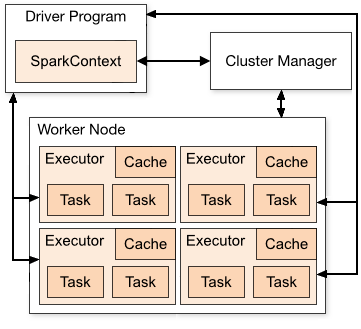
\includegraphics[width=0.45\textwidth]{test_architecture.png}
  \caption{The simple architecture used during the majority of our tests}
  \label{fig:test_architecture}
\end{figure}

\subsubsection{Program Parameters}

At all time, unless specified otherwise, the program parameters will be kept at their default value, so that differences in parameters will never be reflected in our performances.\newline

An exception to that rule is the 'maxPatternLength' parameter of Spark, since its default value of 10 doesn't fit our purpose. We will use INTEGER.maxValue instead, so that every solution pattern in our datasets may always be outputted.\newline

Should we add other optional functionalities, we will also make sure their default parameter has no effect on the measured performance, and always use theses default value unless specified otherwise in our tests. \newline

Later in our paper, we will also compare the performance of our final implementation under default and optimal parameters.

\subsubsection{Number of Partitions}

As seen previously in Figure \ref{fig:hadoopVSspark}, Spark's performance may vary greatly depending on the number of partitions created from the Input dataset. Should too much be created, the algorithm will lose considerable amount of time switching its execution between partitions. Should it be too little, scalability will be affected as executor will need to hold large partitions in memory. Spark's shuffler may even crash in the direst cases. \newline

We will thus keep a constant number of partitions for each dataset. So that our performances can remain completely comparable. The number of partitions was specifically chosen for each dataset, as to guarantee good performances and the complete absence of shuffler crash due to too large partitions. \newline

The number of partitions created for each dataset are displayed in Table \ref{tab:numPartitions}. As you can see, the number of created partition is closely related to the database's size.

\begin{table}[h]
  \centering
  \begin{tabular}{| c | c | c |}
  	\hline
  	Dataset & File size (Ko) & Number of partitions \\
  	\hline
  	BIBLE & 3065 & 250 \\
  	\hline
  	FIFA & 2594 &300\\
  	\hline
  	Kosarak-70 & 2166 & 250\\
  	\hline  
  	LEVIATHAN & 713 & 100\\
  	\hline
  	PubMed & 1646 & 200\\
  	\hline
  	protein & 126046 & 5000\\
  	\hline
  	slen1 & 5400 & 500\\
 	\hline 
  	slen2 & 6896 & 500\\
  	\hline
  	slen3 & 39654 & 1000\\
  	\hline
  \end{tabular}
  \caption{Number of partitions used during performance tests}
  \label{tab:numPartitions}
\end{table}

\subsubsection{Measurement Span}

For our performance tests, we will measure not only the running time of our algorithm, but also its pre-processing and dataset loading performances. The aim being to develop a new implementation that entirely surpasses the old one. \newline

\section{The PrefixSpan Algorithm}

TODO ? Is it necessary

\section{PPIC and Spark's Original Implementation}

In this section, we will explain the original implementation of PPIC and Spark, and then compare their performance.

\subsection{Spark's original Implementation}

Spark's algorithm can be separated in four stages :

\begin{enumerate}
\item \textbf{Pre-processing :} The goal of this stage is to replace each item of the sequence database by an unique ID, to separate itemSets by a zero delimiter, and to clean the database from unfrequent items. \\
For example, the sequence <(ABD)(ABC)A> will become 0120123010, assuming only items A, B and C are frequent in the sequence database.
\item \textbf{Scalable execution :} The core of the algorithm. Its execution consist in extending prefixes through a three sub-stage process, starting from the empty prefix.
	\begin{enumerate}
	\item First, a large prefix is projected on the database. If there is no prefix to project, the scalable execution comes to an end and the solutions will be returned.
	\item Then, from the set of supporting sequences, we discover symbols that can extend the current prefix. If no such extension exists, we try the next large prefix.
	\item Finally, for each possible symbol extension, we extend the prefix. we then determine how long further expanding each extended prefix may take by calculating the projected database size. Depending on the calculated projected size and of the value of a user defined parameter, we then either further extend this prefix using another iteration of scalable execution, or store it for use in the local execution stage. 
	\end{enumerate}
\item \textbf{Local execution :} The local execution is completely similar in its implementation to the scalable execution. Its only use is in improving the algorithm's performance by calculating all extensions from a Prefix locally, instead of doing so while shuffling information around the scalable architecture. \\
This stage is only launched once all large prefixes have been extended sufficiently, making the databases needed for future extensions small enough. Depending on the parameters inputted by the user, this stage may be skipped. TODO: add performance difference of keeping database on shuffle file.
\item \textbf{Post-processing :} During the post-processing step, we translate back the unique IDs into the item they each represented. Then we send back the collected results to the user.
\end{enumerate}

During the prefix projection phase of the scalable and local execution, the algorithm will also detect which item-sets in the sequence comply with what has already been projected and can still be extended in some way. Storing such items positions in a 'partial projection' list. \newline
That way, if we are projecting an item-set containing multiple symbol from a prefix, until the end of that item-set, the items projection phases will know where to search possible extensions, preventing the algorithm from having to search the whole sequence. \newline
Also, should we be computing a single-item pattern mining problem, no partial start would be created and kept in memory, since the algorithm automatically detect that those item-sets cannot be extended. \newline

If the item-set end, the full remains of the sequence, from the earliest partial position recorded, will have to be searched. During this search, new potential partial projection will be recorded, and the old ones will be discarded. \newline

During the prefix extension phase, the current partial projection will also be used to find extensions of the current itemset quicker. The remainder of the database will also be searched, but only for extension that starts new itemsets. \newline

An example of a fully scalable execution from this algorithm can be found in figure \ref{fig:spark_exec_example} \newline

\begin{figure}[h]
\centering
\scalebox{0.55}{
\begin{forest}
for tree={
  draw,
  minimum height=2cm,
  anchor=north,
  align=center,
  child anchor=north
},
[{Input sequences : \\ <(ADB)(ABC)(A)> \\ <(ABC)A>}, align=center, name=SS
  [{Pre-processed sequences : \\ <0120123010> \\ <0123010>}, name=PDC
  	[{Empty prefix projection : \\ <|0120123010> \\ <|0123010> \\ Partial starts : \\  \textrm{[]} \\ \textrm{[]} \\ Extensions found : \\ \textrm{[01, 02, 03]}},
  		[{Projecting 01 : \\ <01|20123010> \\ <01|23010> \\ Partial starts : \\  \textrm{[4]} \\ \textrm{[]} \\ Extensions supported : \\ \textrm{[2, 3, 01]}},
  			[{Projecting 0101 : \\ <012012301|0> \\ <012301|0> \\ Partial starts : \\  \textrm{[]} \\ \textrm{[]} \\ Extensions supported : \\ \textrm{[]}}]
  			[{Projecting 013 : \\ <0120123|010> \\ <0123|010> \\ Partial starts : \\  \textrm{[]} \\ \textrm{[]} \\ Extensions supported : \\ \textrm{[01]}},
  				[{Projecting 01301 : \\ <012012301|0> \\ <012301|0> \\ Partial starts : \\  \textrm{[]} \\ \textrm{[]} \\ Extensions supported : \\ \textrm{[]}}]
  			]
  			[{Projecting 012 : \\ <012|0123010> \\ <012|3010> \\ Partial starts : \\  \textrm{[5]} \\ \textrm{[]} \\ Extensions supported : \\ \textrm{[3, 01]}},
  				[{Projecting 0123 : \\ <0120123|010> \\ <0123|010> \\ Partial starts : \\  \textrm{[]} \\ \textrm{[]} \\ Extensions supported : \\ \textrm{[]}},
  					[{Projecting 012301 : \\ <012012301|0> \\ <012301|0> \\ Partial starts : \\  \textrm{[]} \\ \textrm{[]} \\ Extensions supported : \\ \textrm{[]}}]
  				]
  				[{Projecting 01201 : \\ <012012301|0> \\ <012301|0> \\ Partial starts : \\  \textrm{[]} \\ \textrm{[]} \\ Extensions supported : \\ \textrm{[]}}]
  			]
  		]
  		[{Projecting 03 : \\ <0120123|010> \\ <0123|010> \\ Partial starts : \\  \textrm{[]} \\ \textrm{[]} \\ Extensions supported : \\ \textrm{[01]}},
  			[{Projecting 0301 : \\ <012012301|0> \\ <012301|0> \\ Partial starts : \\  \textrm{[]} \\ \textrm{[]} \\ Extensions supported : \\ \textrm{[]}}]
  		]
  		[{Projecting 02 : \\ <012|0123010> \\ <012|3010> \\ Partial starts : \\  \textrm{[5]} \\ \textrm{[]} \\ Extensions supported : \\ \textrm{[3, 01]}},
  			[{Projecting 0201 : \\ <012012301|0> \\ <012301|0> \\ Partial starts : \\  \textrm{[]} \\ \textrm{[]} \\ Extensions supported : \\ \textrm{[]}}]
  			[{Projecting 023 : \\ <0120123|010> \\ <0123|010> \\ Partial starts : \\  \textrm{[]} \\ \textrm{[]} \\ Extensions supported : \\ \textrm{[01]}},
  				[{Projecting 02301 : \\ <012012301|0> \\ <012301|0> \\ Partial starts : \\  \textrm{[]} \\ \textrm{[]} \\ Extensions supported : \\ \textrm{[]}}]
  			]
  		]
  	]
  ]
]
%\node[anchor=west,align=left]  at ([xshift=-2cm]MS.west) {Level 3\\Criteria};
\end{forest}}
\caption[An example of Spark's execution]{
	\tabular[t]{@{}l@{}}
		A simple execution of Spark's algorithm.\\
		The solutions are the projected prefixes (except the empty prefix)
	\endtabular
}
\label{fig:spark_exec_example}
\end{figure}

TODO - Should I add some pseudo code ? \newline
  	
\begin{itemize}
  \item[NB:] During our first analysis of Spark's pre-processing stage, we noticed a small inefficiency in the cleaning of the database's sequences. When multiple itemsets were fully cleaned of their item, the algorithm had a tendency of creating sequences of zero delimiters, as the algorithm still delimited empty itemsets.

Although the internal representation was still correct and results weren't modified, those trailing zeroes substantially slowed the algorithm down.
The performance improvement of this small correction is reflected in the annexes, figure \ref{spark_preprocessing_fix}.

Later, this small correction was proposed to Spark's community and quickly accepted into the default implementation. In the remains of this paper, we will thus consider this corrected version which has been approved by the community as the original algorithm for Spark, and compare our performance improvement with this corrected version as the basis.
\end{itemize}

\subsection{PPIC's Original Implementation}

PPIC's execution can be separated in two stages :

\begin{enumerate}
\item \textbf{Pre-processing :} In this first stage, we first clean the received sequences from unfrequent items, renaming them into unique ID's. Three matrices are then build from the sequence database :
	\begin{enumerate}
		\item The 'first-position' matrix : A \#SDB*N sized matrix allowing O(1) jumps to the first occurrence of a given item. 
		\item The 'last-position' matrix : A  \#SDB*N sized matrix allowing O(1) check for the presence of a given item in the remains of a sequence.
		\item The 'interesting-position' matrix : A matrix with the same size as the original sequence database, but whose content are changed from the items forming those sequences, to the positions of the next 'interesting' item. That is the next position where an item last appears in a sequence. \\ Although, at first glance, this matrix may seem redundant with the last-position matrix, its purpose appears when one realise that to achieve the same goal a whole columns of the last-position matrix would have to be checked. Similarly, keeping only this matrix would also be less efficient, since there would be no way to efficiently check if an item is present in the remains of a sequence. Both matrices are thus needed to achieve the greatest efficiency gain. 
	\end{enumerate}
	It is interesting to note that, since PPIC has only been implemented for single-item pattern mining problem. No delimiter are inserted into the cleaned sequence database, making its representation more compact than in Spark's prefix-span. \newline
	
	The pre-processing stage will also take care of adding multiple constraint, depending on the wishes of the user. Thus restraining the solution space as desired and improving performances at reaching specific solutions.
	
\item \textbf{Execution :} Once the pre-processing is finished, the algorithm will truly start to run. Using the three matrices, prefixes will then be extended efficiently using a DFS approach possible thanks to trailing. Which is more efficient than a BFS approach were multiple copies of the database would need to be kept. Memory consumption during the execution will thus be minimal. \newline

Each time a valid solution is found. That is, a solution that satisfy all constraints. The execution will be momentarily interrupted. The solution will then be translated back to the items name corresponding the recorded ID's. \newline

Once the solver determines that no further solution can be found under the specified constraints. The execution will terminate, and all resulting pattern will be returned.
\end{enumerate}

TODO - Speek more about how the execution is happening \newline
TODO - Add image  + explanation of sequence selection
TODO - Add exampless
TODO - Should I add some pseudo code ?

\subsection{Performance Comparison}

Now that we understand both algorithms better, the time has come to compare their performance under similar resources. Since PPIC's is neither scalable nor concurrent, we will exceptionally use and even simpler architecture for our test on Spark by restraining our worker to a single executor. \newline

As you can see in Figure \ref{fig:originalAlgorithmPerformances}, given the same resources, PPIC greatly overcomes Spark on most datasets. But, although it completely outperforms Spark's implementation on sparser dataset like protein, it fails to do so on denser datasets like Kosarak-70. Especially when the minimal number of supporting sequence is large, and much of the dataset can be cleaned during the pre-processing stage. \newline

We can also notice that PPIC's performance are far more stable, and that running additional tests for a smaller amount of minimal support may even show on inversion on denser datasets like PubMed.\newline

\begin{figure}[h]
  \centering
  \includegraphics[width=0.9\textwidth]{originalAlgorithm.png} \\
  \danger  Test realised on a simplified architecture \danger \\
  \begin{tabular}{c l}
  	 & \\
  	\textbf{PPIC :} & 1 thread  with 10G memory \\
  	\textbf{Spark :} & 1 driver + 1 worker with 1 executor. 10G memory each
  \end{tabular}
  \caption{Original performances of PPIC and Spark}
  \label{fig:originalAlgorithmPerformances}
\end{figure}

\section{Improving the Performances}

\subsection{A First Implementation}

Now that we observed the original performances of both algorithms, the time has come to design a first scalable implementation. \newline

As mentioned earlier in this paper, Spark's algorithm was composed of two different execution stages. We thus analysed each stage independently to understand how CP technique could improve their implementation. Although we rapidly discovered that the scalable stage could hardly be modified to efficiently incorporate CP techniques, we realised the local execution stage could be significantly improved. \newline

In fact, the entire local execution could be easily replaced by a CP based algorithm, for single-item pattern mining problems where PPIC is applicable, we could even use a nearly identical implementation. Only the pre-processing needed to be modified as to fit Spark's middle-put. \newline

We thus quickly implemented this change, also adding a simple boolean to specify whether PPIC could be used on the input dataset, and measured the difference in performance displayed in figure \ref{fig:first_scalable_CPbased_implementation}. To this graph, we also added PPIC's performance as we judged this new implementation was closely linked, and that disposing of a comparison may be interesting, please remember PPIC's performance were measured with lower resources than our other performances on this graph.  \newline

\begin{figure}[h]
  \centering
  \includegraphics[width=0.9\textwidth]{first_implementation.png}
  \danger PPIC's performance were still measured using a single thread and 10G of memory \danger \\
  Other performances represented in this graph were measured using the 4-executor test architecture previously described.
  \caption{A first implementation that makes PPIC scalable}
  \label{fig:first_scalable_CPbased_implementation}
\end{figure}

As you can see, this first implementation which simple merges the two algorithm is already much more efficient on single-item pattern problems than Spark's original algorithm. We can however notice than the single-thread execution of PPIC sometimes overcome our new scalable implementation. The worst such case being protein, a dataset on which PPIC remain far superior despite the lower resource it disposes, which may appear disconcerting at first glance. \newline

Another disconcerting thing to notice may be the relative flatness of PPIC's performance measurement. Making it seem as if the decrease in amount of required support isn't really felt by the algorithm, on Kosarak and PubMed their performance remain worse by a 10x factor which cannot be explained by the lack of resources alone. \newline

But, in truth, those difference in performance can be perfectly explained. They result from three major factors :
\begin{enumerate}
\item First, the pre-processing of the original PPIC algorithm wasn't implemented efficiently, probably since only execution time were compared on PPIC's original paper. PPIC's true efficiency was thus brought down, while our new implementation wasn't, since this pre-processing was rewritten from scratch to fit Spark's middle-put. This time, with efficiency in mind. Explaining the slow, yet stable, performances of PPIC on datasets like Kosarak.

\item Second, as explained earlier, three matrices are built from the original sequence database before the beginning of PPIC's execution. However, in PPIC's original implementation, those matrices could be very large. As their size depends not only on the number of sequences, but also on the number of unique item present in the input database. \newline
	
	However, our first-implementation surprisingly solved this problem. Since only the interesting parts of the sequence database are kept before launching the local execution, many items and sequences which appeared in the initial problem don't appear during the local execution. For each sub-problem treated in the local execution, the constructed matrices will thus be much smaller in size. Which explain further our new implementation's efficiency gain on dataset with large amount of distinct items.
	
\item Finally, our third major factor is a major inefficiency that comes as a by-product of scalability. It appear mostly on smaller datasets composed of a small number of repeated symbols, such as our protein dataset. In those cases, since the various sub-problem created before our local execution are actually very similar to each other, our new implementation will lose and important amount of time recreating the three input matrices before launching computations on those nearly identical sequence databases. While the original PPIC implementation would create those matrices once and use them through the reminder of the execution. \newline

Sadly, this problem cannot be dynamically fixed without seriously affecting scalability or efficiency, as it would require us to compare the projection of multiple prefixes. This means that, either we would have to project the prefixes multiple time to obtain the results of those comparison, either we would project it once and keep multiple version of the database during comparison, which would be a disaster for memory consumption and scalability.\newline

Fortunately, although a complete dynamic fix of the problem is unpractical for the implementation of a scalable and efficient solution. It is possible to give users the possibility to reduce or even negate the effects of this by-product inefficiency, through giving them control over the amount of sub-problem created. Since the less such sub-problems, the less those matrices will need to be recalculated. \newline

In fact, Spark's implementation already contains a way to control the number of sub-problems created, thanks to the 'maxLocalProjDBSize' parameter. Stopping further sub-problem creation from problems that are already below the inputted parameter value in size. A more direct and precise way to control the amount of generated problems wouldn't be superfluous, but its addition will be studied later in this paper.

\end{enumerate}

On the other hand, we can notice that multi-item performance haven't changed much, if at all. Which is normal since the modification made only concerned single-item problems. \newline

TODO : Should I put an emphasis on the important part below by putting it in its own section ? \newline

Now that we understand where those performances come from, we need to find how to improve them further. In that endeavour, we identified three options that needed to be studied:

\begin{enumerate}
	\item Improve the link between Spark's middle-put and PPIC's input. The easiest option, but also the most promising, since both algorithm have been separately optimised in terms of performances.
	\item Improve Spark's performances by incorporating more idea's from pattern mining.
Which would improve both the scalable execution and the original local execution component of Spark. Thus improving performances on both single and multi-item pattern problems.
	\item Developing a new version of PPIC which can efficiently be applied to multi-item pattern. Making CP usable for every local execution opportunity, and improving performances.
\end{enumerate}

Additionally to those performance improving options, we also decided to prove that PPIC's modularity can be conserved through the addition of more functionalities.

\subsection{Improving the Link}

\subsubsection{Adding Functionalities \& Improving Middle-put Translation}

From the first implementation presented previously, we set out to implement new functionalities and improve the link between Spark's middle-put and PPIC's input. \newline

First, we implemented four new functionalities :
\begin{enumerate}
	\item Unbounded max pattern length : Although Spark's implementation already disposed of a way to control the maximum length of a pattern, no special value existed to allow unlimited max pattern length. We thus added this minor functionality.
	\item Min pattern length : We added a functionality to specify the minimal length a pattern should have before being considered solution.
	\item Limit on the maximal number of item per item-set : This functionality was added so that user could better control the outputted results. Supposing an hypothetical business would like to find all sequences of item bought in pair in a dataset, it would have no need for solutions where item-sets are larger than two. We can thus stop searching for further item-set extensions once the limit has already been reached, and de-facto, improve our algorithm performances for returning those specific solution.
	\item Soft limit on the number of sub-problems created : By default inactivated, this parameters is enabling far better performance on protein like datasets where projected databases tend to be rather similar in sub-problems. Its implementation is a simple check at the beginning of each iteration of the scalable algorithm. If the number of sub-problem created is larger than the user inputted value, the implementation will forcefully put an end to the scalable stage, and switch to a local execution on each worker.\newline
	 As you can see in Figure \ref{fig:sub_problem_limit}, performance improvement are only observed on the protein, Kosarak and slen2 datasets, but the increase in performance is significant. The problem being that the loss of performance on other datasets is generally even more significant. This loss in performance comes from large differences in sub-problems sizes appearing due to the forced local execution. Since the largest problems tend to be created and processed last, only a few executor have problems to work on toward the end of the execution. The remaining executor staying idle for the reminder of the local execution stage. Moreover, those remaining problems take a very long time to compute, greatly slowing down the measured performance. \\
	 As is, this parameter should be used with extreme care. However, we will consecrate a section to studying possible improvement of its performances later in this paper. TODO link to that section.
\end{enumerate}

While these additions did not have any measurable impact on performances at their default value, they still allowed better control of the search space. Proving a certain level of modularity was easily kept from the original CP based implementation. In all the following graph, unless specified otherwise, those parameters will be kept to their default value, as to make sure they do not interfere with the observed efficiency gain/loss. \newline

We then looked into improving our performances, leading to the implementation of two changes. \newline

\begin{figure}[h]
  \centering
  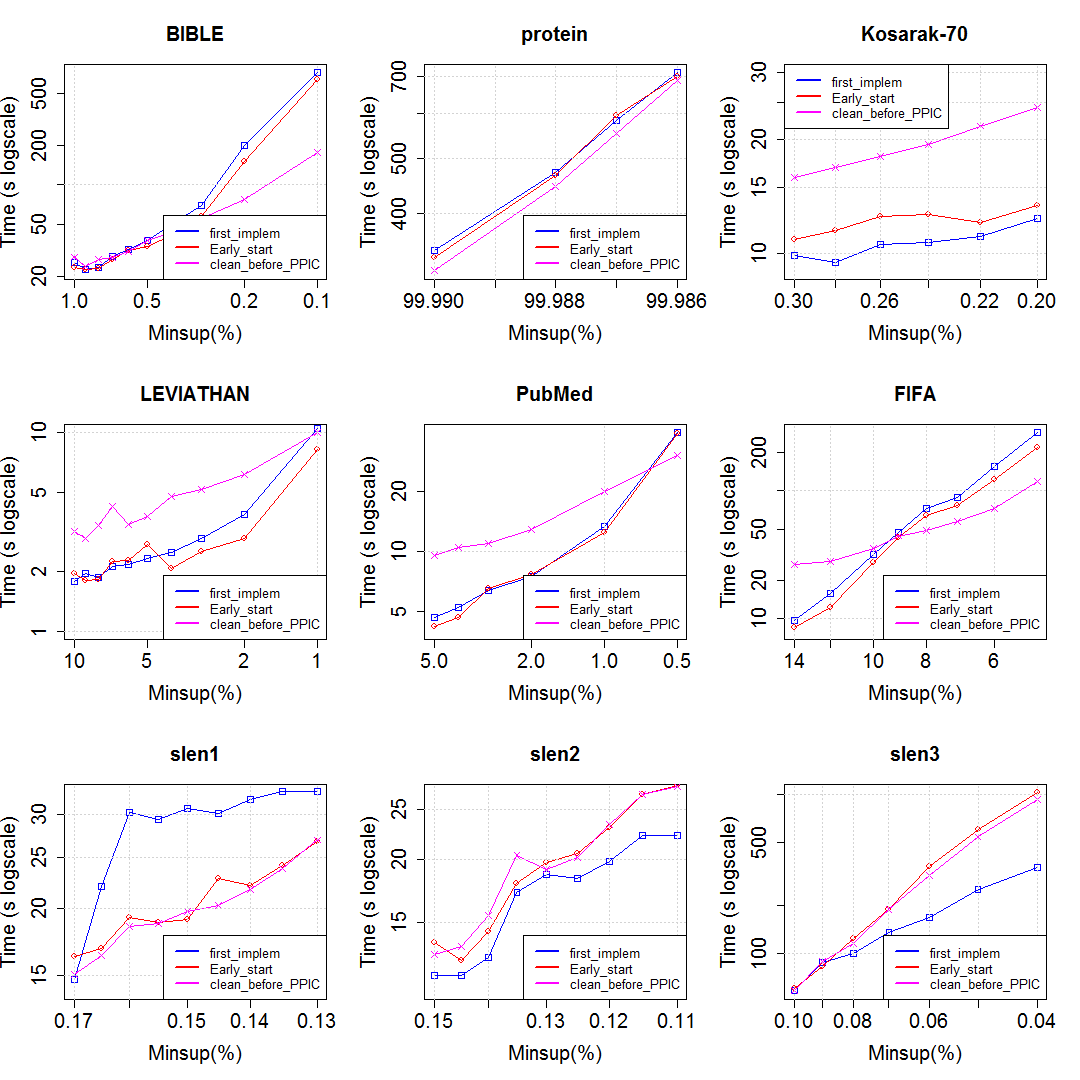
\includegraphics[width=0.9\textwidth]{new_functionalities.png}
  TODO - Should I put another version of the graph without log-scale. The improvements seem downgraded due to that scale here.
  \caption{The performance impact of adding new functionalities}
  \label{fig:new_functionalities_perf}
\end{figure}


First, during its pre-processing, Spark cleans unfrequent items from the database, finding frequent items in the process. In the original implementation, those frequent items are then discarded, and pattern searches are launched starting from an empty prefix. We thus decided to try keeping those frequent items, and passing them as starting prefixes to the various worker. Hereby removing the first and longest iteration of the algorithm. The performance obtained by implementing this change and the preceding 4 functionalities are reflected on the red line of Figure \ref{fig:new_functionalities_perf}.
\newline

As you can see, very small gain in time are generally made. At the exception of the Kosarak-70 and slen-2 datasets, which posses a lot of item but become quite small once cleaned. We believe those small loss of performance are due to the delay needed to transfer the already calculated frequent items to the various executor being larger than the time needed to actually recalculate those items from the small cleaned database in a scalable environment. \newline

Despite the inefficiency on those two datasets, we decided to keep this change, as the efficiency gain can be relatively significant on larger datasets like Fifa or Bible. \newline

We then implemented a second change, an additional pre-processing stage before the local execution of PPIC, so that unfrequent items would once again be detected and cleaned. The performance obtained, which can also be seen on figure \ref{fig:new_functionalities_perf}, displayed great performance improvement on harder execution. This additional feature allowing a 3x performance speed-up on the Bible dataset and a 2x speed-up on Fifa. Lesser performance gain were also observed on protein and the latter stages of PubMed. \newline

However, we can observe worsening performances in smaller datasets and in executions with larger minsup values. Theses loss however, pales in comparison to the performance gain observed. Although at first glance they may seem large on log-scale graph, they do not even exceed ten second, while the performance can be counted in hundred of seconds on Bible and Fifa. \newline

The reason behind those performances is fairly simple. The larger the dataset and the lower the minimal amount of support, the longer prefixes will need to be before being executed locally. The larger those prefixes are before local execution, the more items can be cleaned from the sequences, the faster we can search the remain of those very sequences for patterns. Finally, if less items are present in our sequences during our local execution of PPIC, the three matrices needed for PPIC's execution can be created faster. Thus, hastening performance another fold. \newline

However, cleaning sequences comes with a variable cost depending on the database size. If, much like Kosarak, the database only contains uncleanable sequences, performances will be worsened. Of course, since this change is only applied before PPIC, the performance measured on our two slen datasets weren't affected. \newline

In the end, since such large increase in performances were observed, and since so many other improvements needed to be tested, \textbf{we decided to use the performance obtained here as reference for the remainder of this paper}. To allow better comparison of performances gain/losses, all further improvement will thus be added to this version, and tested separately. Finally, by the end of this paper, a final version containing all changes providing performance improvements will be compiled into a single algorithm. Of whose the performances will be tested.

\begin{figure}[h]
  \centering
  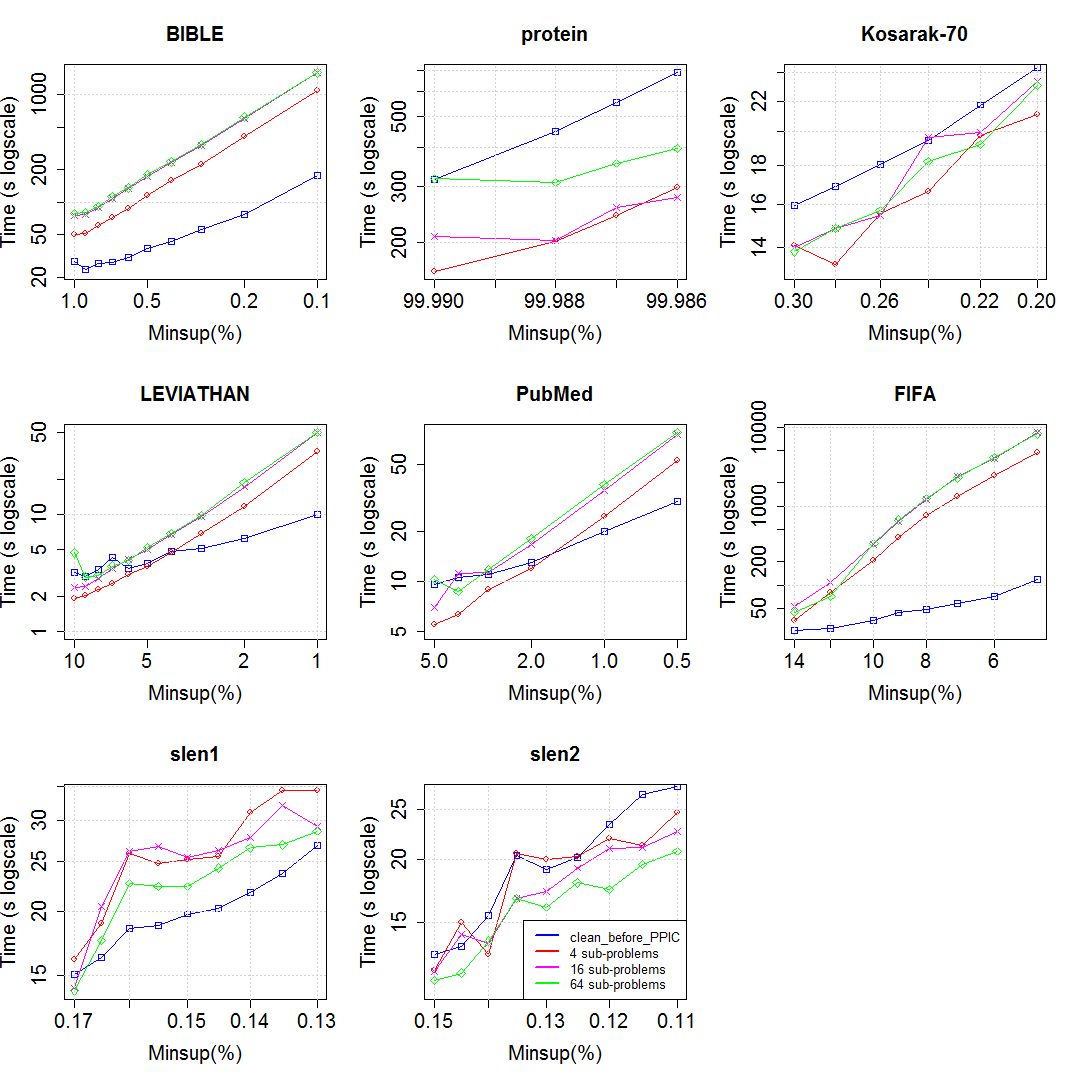
\includegraphics[width=0.9\textwidth]{sub_problem_limit.png}
  \caption{Performance improvement - soft limit on the number of created sub-problem.}
  \label{fig:sub_problem_limit}
\end{figure}

\subsection{Improving Spark}

In this section, we will discuss the improvement we tried to bring to Spark, and the results we obtained. For each improvement, we will first explain its nature and the trade-off's its implementation may encompass.

\subsubsection{Automation of the Choice Between PPIC and Spark's Local Execution}

The first implementation we decided to undertake, was to automatise to choice between PPIC and Spark's local execution. Using the former only for single-item patterns, and the latter for multi-item patterns. Automatic detection being a feature we judged important to implement efficiently, since we judged it was something our user shouldn't constantly be aware of. \newline 

In that endeavour, our first go to was calculating the maxItemPetItemSet argument dynamically during the pre-processing stage. Since it allow us to determine whether we were dealing with single-item patterns, and thus, whether PPIC could be used. \newline

As you can see on figure \ref{fig:maxItemPerItemset_recalculated}.
While this improvement achieved its goal, slight performance degradation were also observed, due to the need for calculating this value. \newline

While, at first, we thought those small loss where worth for this feature, we ultimately decided to discard this change as a more efficient way of doing that exist. As you will see in the next section, it can be implemented in a non performance damaging way.

\begin{figure}[h]
  \centering
  \includegraphics[width=0.9\textwidth]{MaxItemPerItemset_recalculated.png}
  \caption[Automatic detection of item-sets type in dataset]{
  	\tabular[t]{@{}l@{}}
		Performance improvement of recalculating maxItemPerItemset to avoid \\
		search for multi-item extension when unnecessary
	\endtabular}
  \label{fig:maxItemPerItemset_recalculated}
\end{figure}

\subsubsection{Additional Pre-processing Before the Local Execution}

Extending our previous idea of cleaning the sequence database before PPIC's execution, we wondered if cleaning the sequence database before Spark's original local execution could bring similar improvements. \newline

We thus designed a new cleaning process suited both for Spark and PPIC's local execution input. During this process, we also modified the algorithm so that it could automatically detect whether the current sub-problem concerned single-item or multi-item pattern mining, redirecting the execution to the appropriate local execution thereafter. \newline

While creating the new cleaning algorithm, we also discovered more than a few inefficiencies on the old one. Such as the use of ArrayBuffer structure instead of the much more efficient ArrayBuilder, or un-needed extra iteration during the matrices creation. \newline

The new version of the algorithm was thus far more performant on both type of pattern mining problems, as you can see in figure \ref{fig:cleaning_before_local_exec}. \newline

\begin{figure}[h]
  \centering
  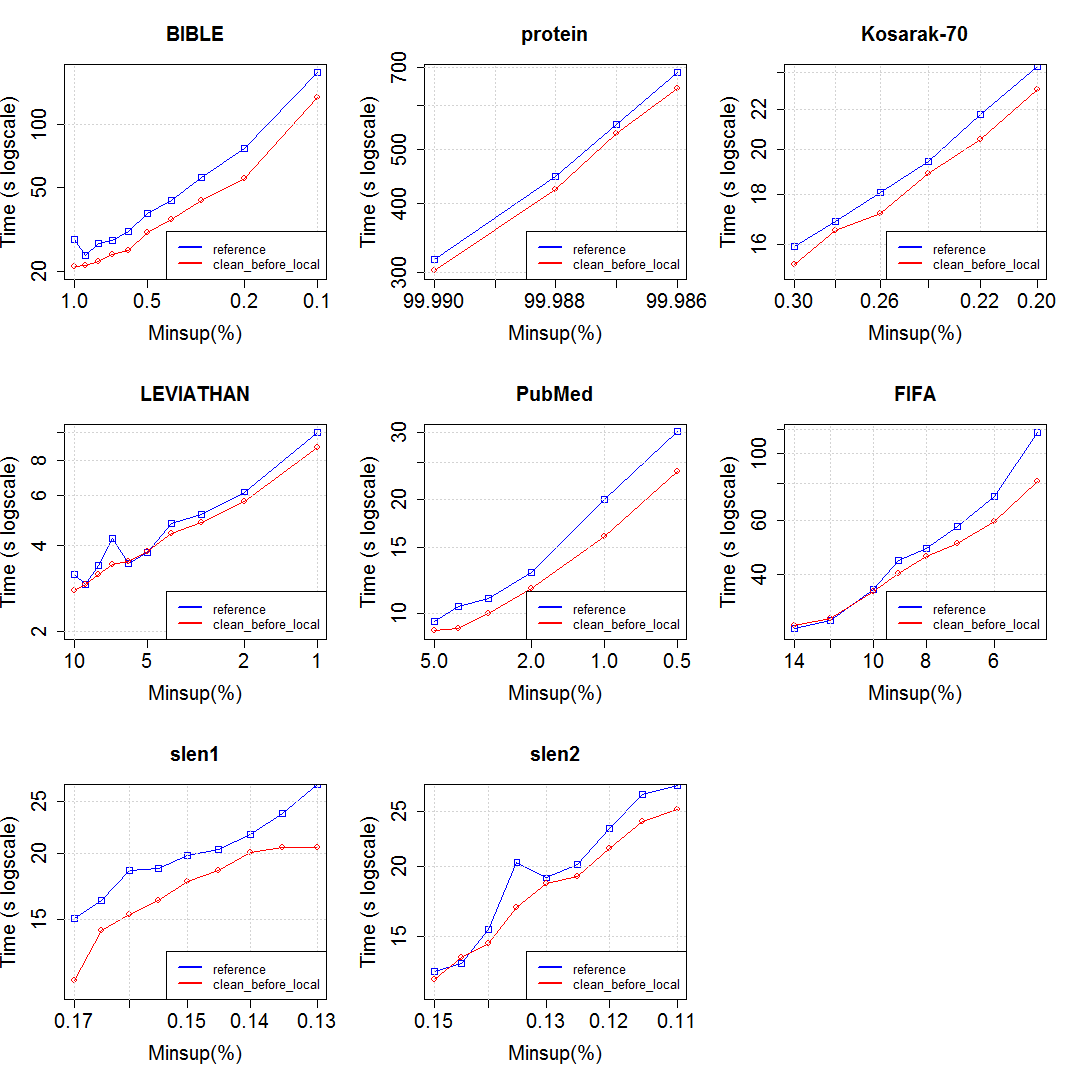
\includegraphics[width=0.9\textwidth]{clean_before_localExec.png}
  \caption{Efficiency gain of cleaning the sequence database before any local execution}
  \label{fig:cleaning_before_local_exec}
\end{figure}

Another advantage of moving our local execution detection to a cleaning stage executed before the local execution was that, should a sub-problem from a multi-item pattern dataset become a single-item pattern problem through cleaning, its local execution can be done through PPIC, thus improving the performances. \newline

For mixed datasets where some multi-item itemsets may rarely appear, this change may thus provide great performance improvement. Sadly those kind of datasets are rarely, if at all, used in the industry. We thus couldn't get our hand on such a mixed dataset to run tests, and compare performances.

\subsubsection{First/Last Position List}

The third idea we had to improve Spark's performances, was to use LAPIN's position list to our advantage. \newline

In Spark's original implementation, the scalable and local stages of the algorithm perform their duty in three phases. First they receive a solution prefix which needs to be extended and project it on the whole database, allowing them to know which sequence support that prefix. Then, in the supporting sequence only, they search for symbols which may extend the prefix. Finally, If some symbols are found and they respect the constraint applied to the solutions, Spark's will save them as solution and try to extend them further. \newline

While this implementation is very efficient in a scalable environment, we thought it could be improved through the addition of position list. More specifically, during the prefix projection phase, we determined it would improve performance if the algorithm knew earlier when a sequence couldn't possibly hold the currently projected pattern, or if the algorithm didn't have to analyse half of the sequence before starting to project this aforementioned pattern. \newline

We thus modified our reference algorithm into three modified version. The first using only a last position list, the second using only a first position list, and the last using both together. We then tested their performance, obtaining the results of Figure \ref{fig:positionListPerf} \newline

\begin{figure}[h]
  \centering
  \includegraphics[width=0.9\textwidth]{positionLists.png}
  \caption{Performance gain of first/last position lists}
  \label{fig:positionListPerf}
\end{figure}

As you can see, the results weren't conclusive. On every single-item dataset but protein, which is a very sparse dataset on which this type of techniques excel, the modified algorithms delivered worse performances than our current reference algorithm. \newline

Those worsening performance appear because the benefit of those additional computation simply do not have time to appear. After being calculated during the pre-processing, they only stay of use during the scalable execution of our algorithm. Since that, before the local execution, the sequence database will be compressed and the positions list will need to be recalculated. \newline

Another reason for those worsening performance would be the transfer time of the calculated positions list, which can be very large depending on the number of frequent items. The delay imposed by their calculation and their transfer through the executor are thus far from negligible. \newline

However, while suffering from the same afflictions, an improvement in performance can be observed on multi-item pattern datasets, where those techniques weren't already in use during the local execution stage, especially on slen1. \newline

For this improvement to show it's full effect, we would thus need to redesign spark's local execution, separating it completely from the scalable stage, so that positions list could only be used locally.
Which also make more sense in a memory consumption point of view, since, on top of the effects being greater, the databases would be smaller and so would be the position lists.

\subsubsection{Specialize Spark's scalable stage for single-item problems}

To improve performance further, we then had the idea separate the scalable execution stage of multi-item and single-item datasets, down to their representation. \newline

We thus implemented a new scalable stage specialised for single-item pattern problems. It's main features being the absence of spacial start and a much more compact database representation without delimiters, since they are in this case unneeded. \newline

A trade-off become however necessary as we now needed to detect in which type of pattern mining problem we were before starting the execution, since we needed to create a different database and simply removing it's delimiters wouldn't have been efficient. \newline

The most efficient way we found to do that was during the frequent detection part of the pre-processing. It however comes at a small variable cost which depends on the database size, as you can see on both slen datasets of Figure \ref{fig:scalable_single_item}. \newline

\begin{figure}[h]
  \centering
  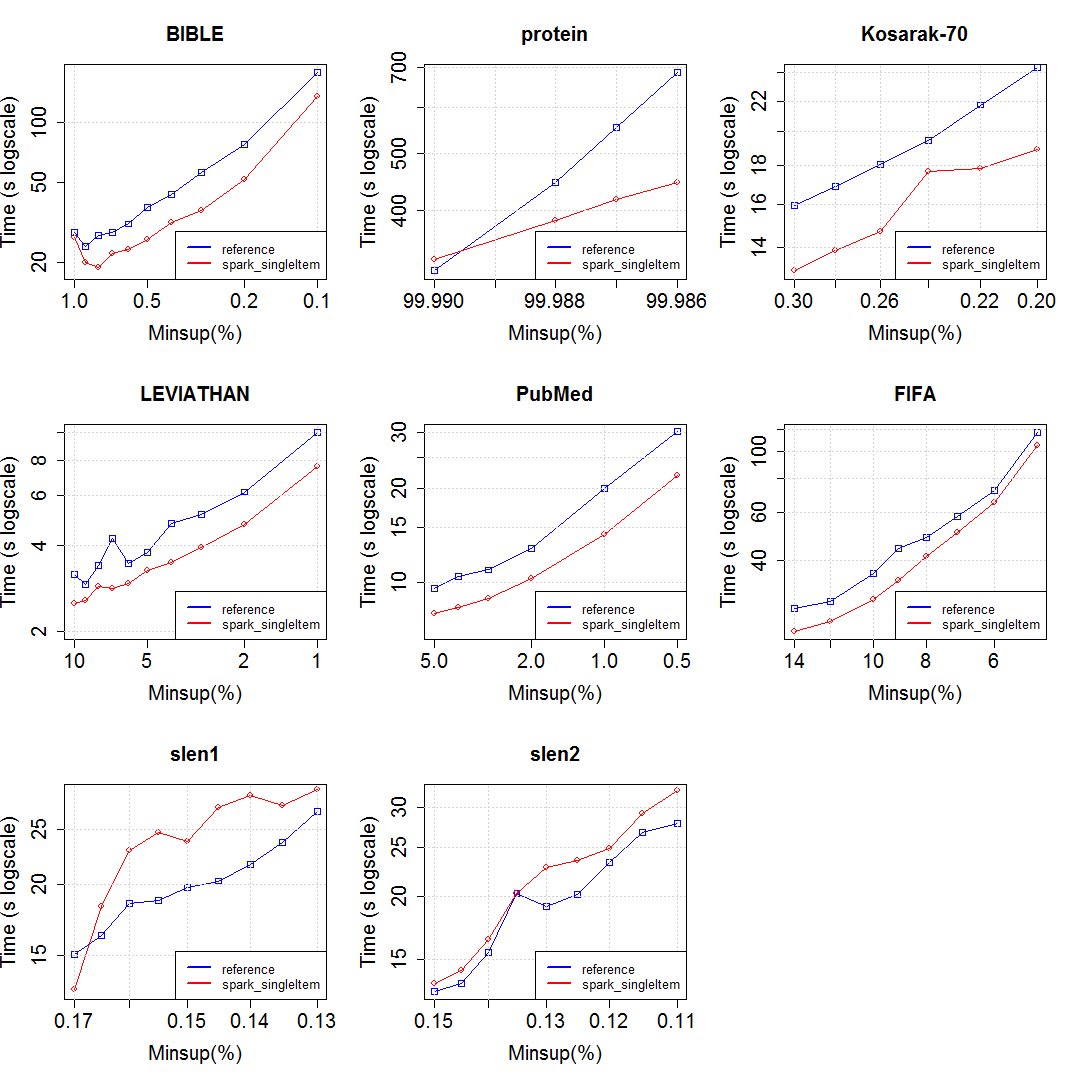
\includegraphics[width=0.9\textwidth]{scalable_single_item.png}
  \caption{Performance improvement of specialising spark's scalable stage.}
  \label{fig:scalable_single_item}
\end{figure}

This small loss in performance on multi-item datasets fortunately remains a small price to pay in comparison to the gains experienced by single-item pattern mining problems, especially on protein where the new scalable algorithm is twice as fast.

\subsubsection{Priority scheduling in local execution}

The final idea we explored to improve Spark's performance, was to modify the order in which sub-problems are computed during the local execution stage. \newline

In the original code, problem are decomposed until they become smaller than a size specified by the 'maxLocalProjDBSize' parameter. As mentioned before, in our reference algorithm, an extension of that idea, the subProblemLimit parameter, was also implemented to allow better control of the number of created sub-problem. \newline

However, we have seen that a consequence of this new functionality is that sub-problems can largely vary in size, making some problem far harder to solve than others. Something would rarely appear in the original version. Coincidentally, we also realised that major drops in performance were experienced if those large problem were solved last, since some executor would be left with nothing to do while other would be stuck with atomic large workload.
\newline

The solution was clear, large problems needed to be solved first in the various executor, so that smaller workload could be shuffled around in the later stage. 

\paragraph{Analysing sub-problem creation}

The piece of code which created the various sub-problems was fundamentally a mapReduce process. The sequences from the original sequence database were one by one projected by different prefixes then mapped to some reducer, depending on the prefix's ID (see Figure \ref{fig:sparkMapReduce}). \newline

\begin{figure}[h]
  \centering
  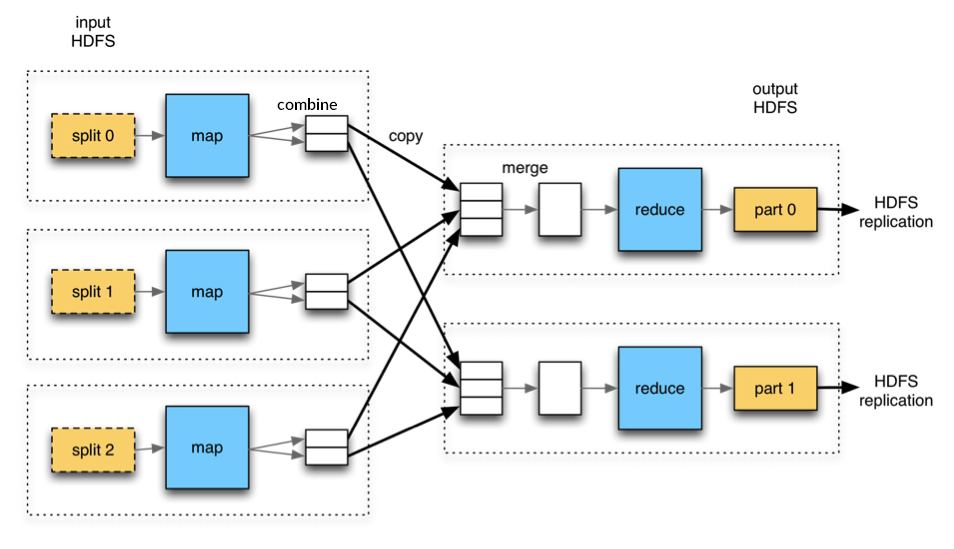
\includegraphics[width=0.8\textwidth]{sparkMapReduce.png}
  \caption{Spark's mapReduce}
  \label{fig:sparkMapReduce}
\end{figure}

\paragraph{Sort sub-problem on the reducer}

We thus concluded a simple solution could be implemented. According to the specification of Spark's sortBy function, the sorting stage will be exacted locally on each reducer. We thus implemented this quick change by adding a simple sort between our map and reduce stage, obtaining the results of Figure \ref{fig:priority_scheduling_performance_comparison}. \newline

\begin{figure}[h]
  \centering
  \includegraphics[width=0.9\textwidth]{priority.png}
  \caption[Naive priority scheduling]{
  	\tabular[t]{@{}l@{}}
  		Performance of a 'biggest problems first' scheduling \\
  		executed through the default sortBy() function of Spark.
  	\endtabular
  }
  \label{fig:priority_scheduling_performance_comparison}
\end{figure}

As you can see, net performance improvements can be observed, especially for Kosarak, protein and slen2, and while BIBLE, FIFA and slen1 suffer from slight performance loss in their later stages, the damage is rather limited in comparison to the otherwise gain. Applying the sort function to the algorithm also isn't too damaging  even when sub-problems aren't limited, as we can see with the red line, it should however be avoid should the algorithm remain as is.\newline

At first glance, this thus looks like a nice little improvement. However, a huge problem remain, as you can see on protein's measurements, the black line lack its fourth point. The reason being a constant crash of the algorithm due to a lack of memory ! \newline

As it turns out, to sort the various sub-problems depending on their size, Spark's need to evaluate and hold in memory all sub-problems assigned to an executor and sort them while keeping those sub-problems either on disk or memory. \newline

Since we forbid our algorithm from accessing the disk during our tests, asserting the 10G of memory given to each executor would be enough, we easily concluded our new implementation consumed more than 10G memory on at least one executor. Something which shouldn't happen in a scalable algorithm which should work on even the smallest configuration ! \newline

We thus had to come up with another solution to sort our sub-problems. One that did not involve computing multiple sub-problem and keeping them in memory..

\paragraph{Sort sub-problem on the mapper}

The answer was obvious, if something could be done, it would be during the mapping phase of the mapReduce. But, despite the multiple attempt at modifying Spark's map function to sort its results, we failed to accomplish our goal without using huge amount of memory.

That is, until we realised the painfully obvious. The mapping function of Spark created sub-problem one by one, following the mapping code and sent them directly to the reducer through the groupBy function, which delivered them in the very same order they were sent. \newline

The solution was thus to change the order in which we created our sub-problem, not to sort them afterwards. The create sub-problems would then be mapped to the reducer and computed in the same order that they were mapped.\newline

Meaning that, should we map the hardest problems first, they would also be executed first. \newline

We thus modified our code to sort our prefixes in descending order through their projected database size, a size which was already computed during the scalable stage of our algorithm, and could simply be stored in the prefix until used to sort. \newline

As expected, sorting a few prefixes uses an insignificant amount of memory in comparison to sorting huge RDD containing complete projected database, while producing equivalent, if not better, performances. This implementation performances were thus a huge success, as you can see on Figure \ref{fig:priority_scheduling_improved}. \newline

\begin{figure}[h]
  \centering
  \includegraphics[width=0.9\textwidth]{priority_final.png}
  \caption{Performance improvement of sorting sub-problems during map stage.}
  \label{fig:priority_scheduling_improved}
\end{figure}

Not only had we obtained our previous boost in performance, we also cling very closely to the performance of the reference algorithm when sorting under Spark's default parameters value in this new extension. \newline

This implementation advantages should thus be kept for the final version of our algorithm, since it allows far better performances when using the correct set of parameters and nearly identical performance for default parameters.

\subsection{Improving PPIC}

Our final implementation attempts, were to create a CP-based implementation to solve multi-item pattern mining problems. Of course, to replace the original local execution, this implementation would need to be more performant than it's predecessor.

\subsubsection{Pushing PPIC's Ideas farther}

TODO - TO REDO ENTIRELY WITH NEW ALGO !9

Our first attempt at creating such an implementation, was to try pushing PPIC's ideas further. \newline

We decided to forgo all three pre-computed matrices, and to change the structure of our sequence database to fill those matrices purposes more efficiently. Instead of an array, we changed each sequence into a map containing unique symbols as key and the various positions of each key symbol as value. 
Additionally, we represented the sequence's symbols positions (including zero delimiter position) by a ReversibleArrayStack structure, thus allowing efficient backtracking through trailing. \newline

This new structure's purpose was to allow us to make distant jumps and checks more efficiently, at the cost of an higher memory consumption. Theorically, finding the next position of a given symbol would be O(1), be this the last or first position of the symbol. Should the symbol's position list be empty, or should the last recorder be smaller than our current position in the sequence, we would also know that no more such symbol were contained in the remains of the sequence. \newline

We thus had good faith our performance could be improved, until we saw the results of our performance tests. As you can see in Figure \ref{multi_map}, the performance were terrible. \newline

While we couldn't see exactly why at first, profiling our algorithm revealed it came from two majors factor. First, to attain the same purpose as the three matrices with our map structure, we needed many more trailing points which had to be backtracked at each step of the search. Regularly generating significant period of time were our algorithm did nothing but backtrack the various sequence of its database. \newline

The second factor was solution pruning. In PPIC, pruning solution from the CPIntVar representing our search space could be done by checking the last positions of each item, quickly asserting that if the start of a sequence was after the last position of an item in a sequence, the sequence was no longer supporting the item. \newline

Here, however, the situation was different. To efficiently prune a multi-item pattern problem, checking last positions was no longer sufficient. To prune efficiently, each itemSet now needs to be checked so that its possible extensions could be deemed supported.

\begin{figure}[h]
  \centering
  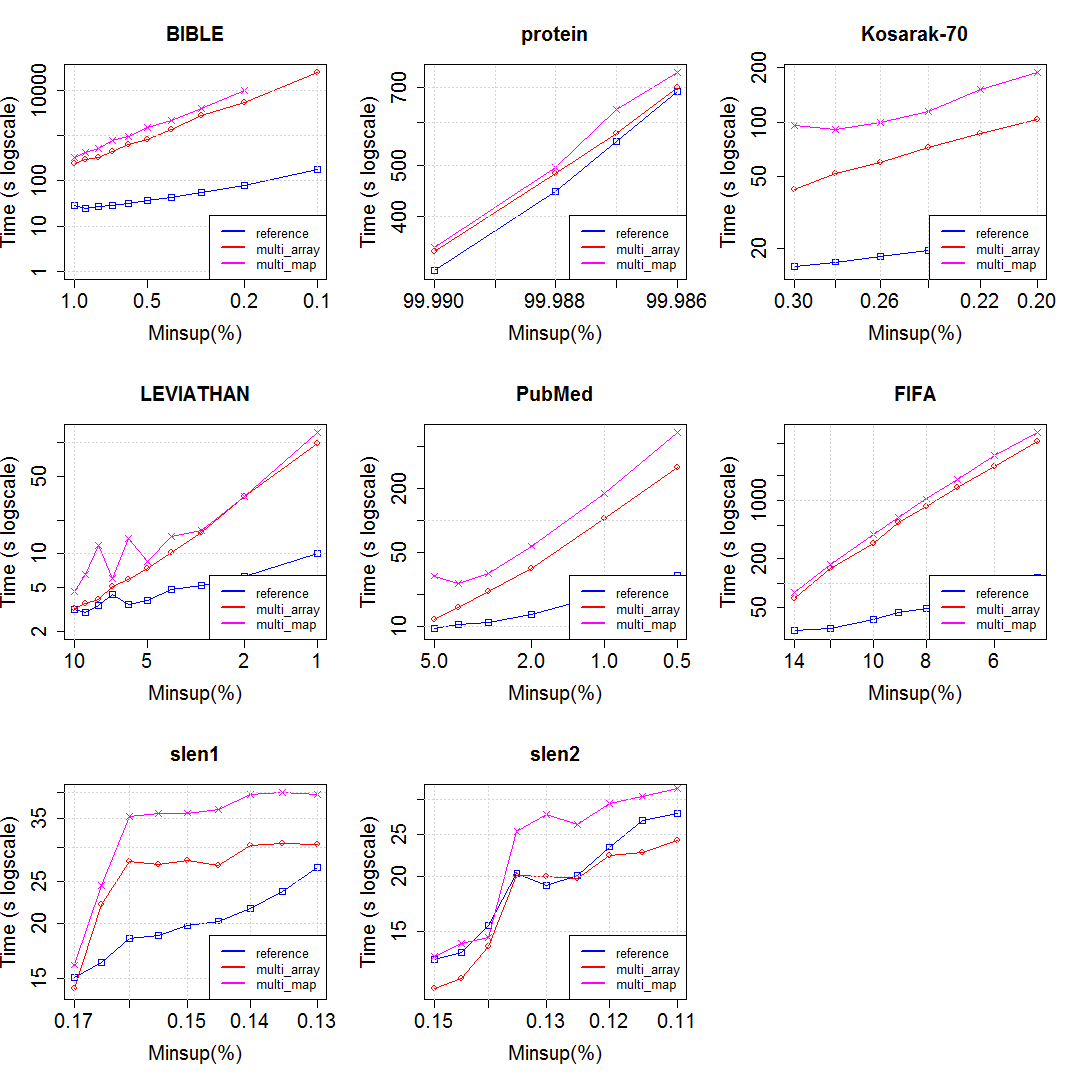
\includegraphics[width=0.9\textwidth]{multi_item_cp.png}
  \caption[PPIC with a map structure]{
  	\tabular[t]{@{}l@{}}
  		Performance of a CP based algorithm replacing \\
  		all three pre-processed matrices from PPIC by a Map structure
  	\endtabular
  }
  \label{fig:multi_map}
\end{figure}

\subsubsection{An Implementation Closer to Spark}

TODO - Solve multi-item bug + add partial-start support

\section{Final Version}

TODO - Redo a final version after all other is finished

\section{Scalability Tests}

TODO - On original simple + final implem

\section{Performances Under Optimal Parameters}

TODO - Only on final version and if result relevant.

\section{Conclusion}

TODO - $\sim$ A page of content

\section{Annexes}

TODO : Add code of all implementation ? Only main ones ?

TODO : Table des abbréviations + symbols !

TODO : Remerciement/Acknoledgement + pas oublier de remercier les serveurs CECI

\subsection{Additional Performance Comparisons :}

\begin{figure}[h]
  \centering
  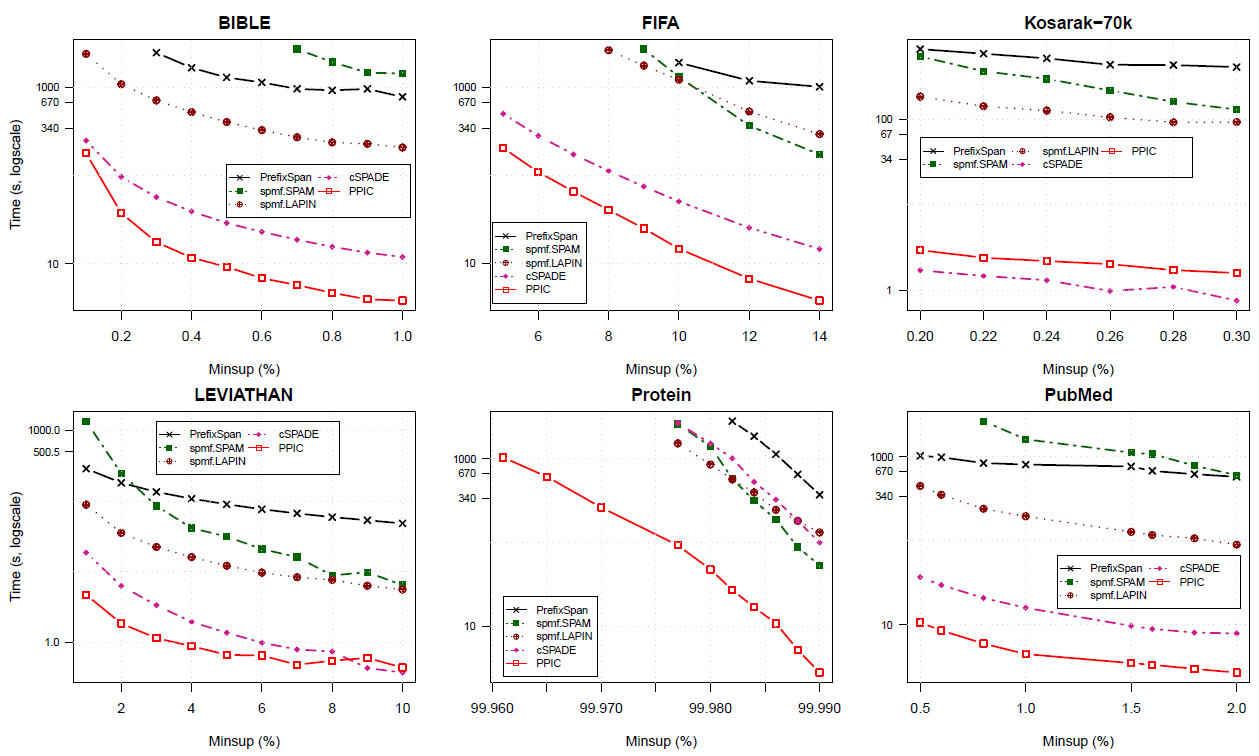
\includegraphics[width=1\textwidth]{PPICvsSpecialised.png}
  \caption{PPIC's performances VS other specialized algorithm}
  \label{PPIC's perfomance against other specialized implementations}
\end{figure}

\begin{figure}[h]
  \centering
  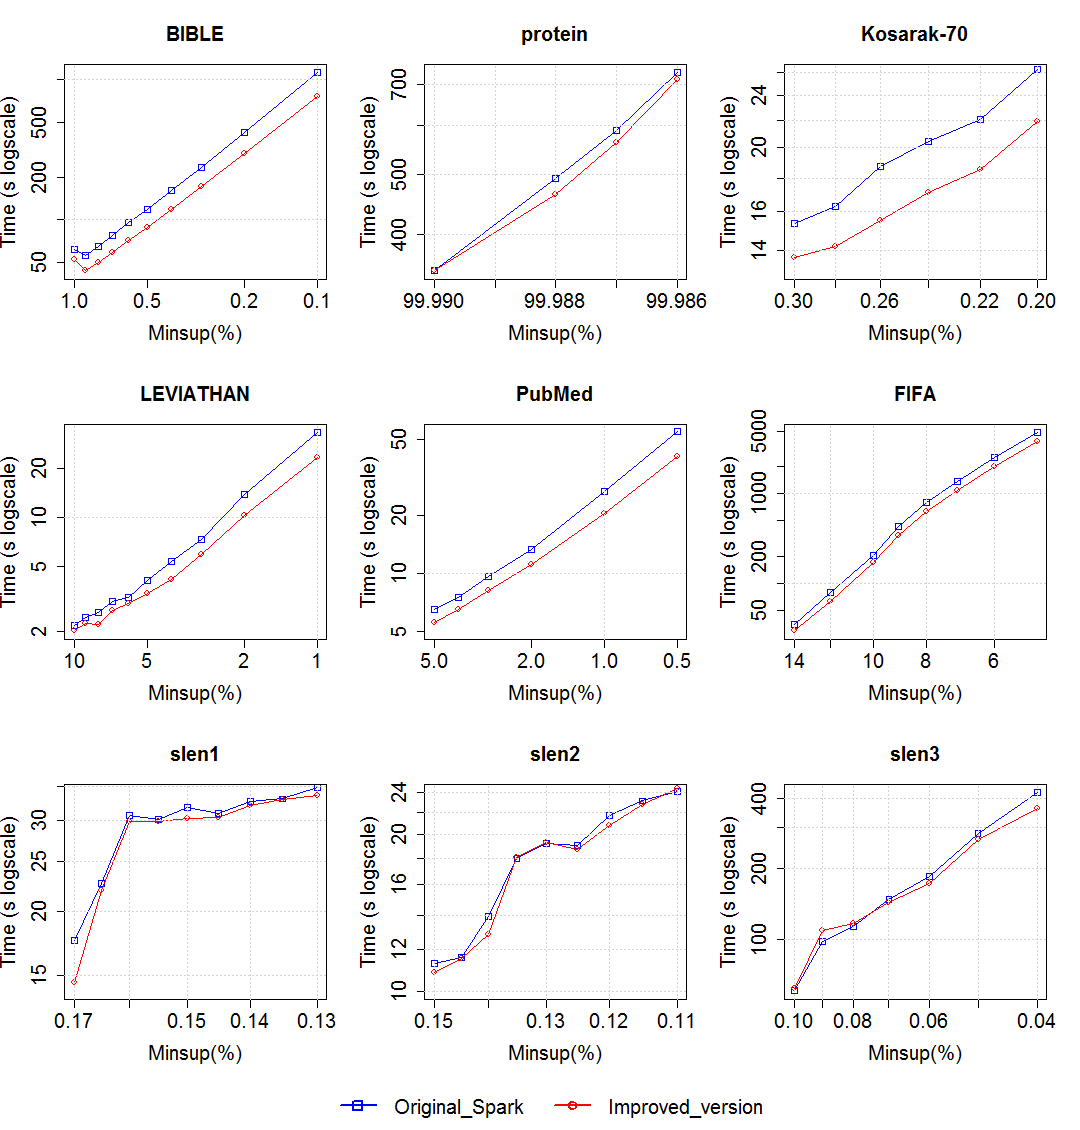
\includegraphics[width=0.9\textwidth]{spark_original_fixed_preprocessing.png}
  \caption{Performance improvement of fixing Spark's pre-processing}
  \label{spark_preprocessing_fix}
\end{figure}

TODO - ADD REFERENCES, CA MANQUE ENCORE
\addcontentsline{toc}{section}{References}
\begin{thebibliography}{9}
\bibitem{RDD} 
Matei Zaharia , Mosharaf Chowdhury , Tathagata Das , Ankur Dave , Justin Ma , Murphy McCauley , Michael J. Franklin , Scott Shenker , Ion Stoica.;
\textit{Resilient distributed datasets: a fault-tolerant abstraction for in-memory cluster computing.}
Proceedings of the 9th USENIX conference on Networked Systems Design and Implementation, April 25-27, 2012, San Jose, CA

\bibitem{Taxonomy} 
Mabroukeh, N. R. and Ezeife, C. I. 2010.;
\textit{A taxonomy of sequential pattern mining algorithms}. 
ACM Comput.Surv. 43, 1, Article 3 (November 2010), 41 pages.

\bibitem{Kemmar_global} 
Kemmar A., Loudni S., Lebbah Y., Boizumault P., Charnois T.;
\textit{Prefixprojection global constraint for sequential pattern mining}.
In: Principles and Practice of Constraint Programming, Springer, 2015

\bibitem{Kemmar_gap} 
Kemmar A., Loudni S., Lebbah Y., Boizumault P., Charnois T.;
\textit{A global constraint for mining sequential patterns with gap constraint}.
CPAIOR16, 2015

\bibitem{itemset_mining} 
Guns T., Nijssen S., De Raedt L. ;
\textit{Itemset mining: A constraint programming perspective}. 
Artificial Intelligence 175(12), 2011. Pages 1951–1983.

\bibitem{PPIC} 
John O.R. Aoga, Tias Guns, Pierre Schaus.;
\textit{An Efficient Algorithm for Mining Frequent Sequence with Constraint Programming},
ECML PKDD 2016: Machine Learning and Knowledge Discovery in Databases, pp 315-330, 2016

\bibitem{Prefix-span} 
Jian Pei, Jiawei Han, Behzad Mortazavi-Asl, Jianyong Wang, Helen Pinto, Qiming Chen, Umeshwar Dayal, and Mei-Chun Hsu;
\textit{Mining Sequential Patterns by Pattern-Growth:
The PrefixSpan Approach}
In: IEEE Transaction on Knowledge and Data Engineering, VOL. 16, Issue 11, Octobre 2004.

\bibitem{LAPIN} 
Zhenglu Yang, Yitong Wang, Masaru Kitsuregawa;
\textit{LAPIN: Effective Sequential Pattern Mining Algorithms
by Last Position Induction for Dense Databases}.
International Conference on Data Engineering, 2005

\bibitem{LAPIN-SPAM} 
Yang Z., Kitsuregawa M.;
\textit{LAPIN-SPAM: An Improved Algorithm for Mining
Sequential Pattern.}
In: International Conference on Data Engineering, 2005

\bibitem{Bonchi}
Francesco Bonchi, Claudio Lucchese
\textit{Extending the state-of-the-art of constraint-based pattern discovery},
Data and Knowledge Engineering, 60 (2) (2007), pp. 377-399

\bibitem{CPforItemSetMining}
Luc De Raedt, Tias Guns, Siegfried Nijssen;
\textit{Constraint programming for itemset mining};
Proceeding of the 14th ACM SIGKDD International Conference on Knowledge Discovery and Data Mining, ACM (2008), pp. 204-212

\bibitem{CPforDataMining}
Luc De Raedt, Tias Guns, Siegfried Nijssen
\textit{Constraint programming for data mining and machine learning}
Proceedings of the Twenty-Fourth AAAI Conference on Artificial Intelligence, AAAI Press (2010), pp. 1513-1518

\bibitem{CPpatternSetMining}
Luc De Raedt, Albrecht Zimmermann
\textit{Constraint-based pattern set mining}
Proceedings of the Seventh SIAM International Conference on Data Mining, SIAM (2007), pp. 1-12

% TODO decide if relevant or not, depending on whether used to compare.
\bibitem{cSPADE} 
Zaki M.J.;
\textit{Sequence mining in categorical domains: incorporating constraints.}
In: Proceedings of the ninth international conference on Information and knowledge management, ACM, pages 422–429, 2000

\end{thebibliography}

\thispagestyle{empty}		
% To suppress header and footer on the back of the cover page
% Back cover page
\backcoverpage
\end{document}
